\documentclass[1p]{elsarticle_modified}
%\bibliographystyle{elsarticle-num}

%\usepackage[colorlinks]{hyperref}
%\usepackage{abbrmath_seonhwa} %\Abb, \Ascr, \Acal ,\Abf, \Afrak
\usepackage{amsfonts}
\usepackage{amssymb}
\usepackage{amsmath}
\usepackage{amsthm}
\usepackage{scalefnt}
\usepackage{amsbsy}
\usepackage{kotex}
\usepackage{caption}
\usepackage{subfig}
\usepackage{color}
\usepackage{graphicx}
\usepackage{xcolor} %% white, black, red, green, blue, cyan, magenta, yellow
\usepackage{float}
\usepackage{setspace}
\usepackage{hyperref}

\usepackage{tikz}
\usetikzlibrary{arrows}

\usepackage{multirow}
\usepackage{array} % fixed length table
\usepackage{hhline}

%%%%%%%%%%%%%%%%%%%%%
\makeatletter
\renewcommand*\env@matrix[1][\arraystretch]{%
	\edef\arraystretch{#1}%
	\hskip -\arraycolsep
	\let\@ifnextchar\new@ifnextchar
	\array{*\c@MaxMatrixCols c}}
\makeatother %https://tex.stackexchange.com/questions/14071/how-can-i-increase-the-line-spacing-in-a-matrix
%%%%%%%%%%%%%%%

\usepackage[normalem]{ulem}

\newcommand{\msout}[1]{\ifmmode\text{\sout{\ensuremath{#1}}}\else\sout{#1}\fi}
%SOURCE: \msout is \stkout macro in https://tex.stackexchange.com/questions/20609/strikeout-in-math-mode

\newcommand{\cancel}[1]{
	\ifmmode
	{\color{red}\msout{#1}}
	\else
	{\color{red}\sout{#1}}
	\fi
}

\newcommand{\add}[1]{
	{\color{blue}\uwave{#1}}
}

\newcommand{\replace}[2]{
	\ifmmode
	{\color{red}\msout{#1}}{\color{blue}\uwave{#2}}
	\else
	{\color{red}\sout{#1}}{\color{blue}\uwave{#2}}
	\fi
}

\newcommand{\Sol}{\mathcal{S}} %segment
\newcommand{\D}{D} %diagram
\newcommand{\A}{\mathcal{A}} %arc


%%%%%%%%%%%%%%%%%%%%%%%%%%%%%5 test

\def\sl{\operatorname{\textup{SL}}(2,\Cbb)}
\def\psl{\operatorname{\textup{PSL}}(2,\Cbb)}
\def\quan{\mkern 1mu \triangleright \mkern 1mu}

\theoremstyle{definition}
\newtheorem{thm}{Theorem}[section]
\newtheorem{prop}[thm]{Proposition}
\newtheorem{lem}[thm]{Lemma}
\newtheorem{ques}[thm]{Question}
\newtheorem{cor}[thm]{Corollary}
\newtheorem{defn}[thm]{Definition}
\newtheorem{exam}[thm]{Example}
\newtheorem{rmk}[thm]{Remark}
\newtheorem{alg}[thm]{Algorithm}

\newcommand{\I}{\sqrt{-1}}
\begin{document}

%\begin{frontmatter}
%
%\title{Boundary parabolic representations of knots up to 8 crossings}
%
%%% Group authors per affiliation:
%\author{Yunhi Cho} 
%\address{Department of Mathematics, University of Seoul, Seoul, Korea}
%\ead{yhcho@uos.ac.kr}
%
%
%\author{Seonhwa Kim} %\fnref{s_kim}}
%\address{Center for Geometry and Physics, Institute for Basic Science, Pohang, 37673, Korea}
%\ead{ryeona17@ibs.re.kr}
%
%\author{Hyuk Kim}
%\address{Department of Mathematical Sciences, Seoul National University, Seoul 08826, Korea}
%\ead{hyukkim@snu.ac.kr}
%
%\author{Seokbeom Yoon}
%\address{Department of Mathematical Sciences, Seoul National University, Seoul, 08826,  Korea}
%\ead{sbyoon15@snu.ac.kr}
%
%\begin{abstract}
%We find all boundary parabolic representation of knots up to 8 crossings.
%
%\end{abstract}
%\begin{keyword}
%    \MSC[2010] 57M25 
%\end{keyword}
%
%\end{frontmatter}

%\linenumbers
%\tableofcontents
%
\newcommand\colored[1]{\textcolor{white}{\rule[-0.35ex]{0.8em}{1.4ex}}\kern-0.8em\color{red} #1}%
%\newcommand\colored[1]{\textcolor{white}{ #1}\kern-2.17ex	\textcolor{white}{ #1}\kern-1.81ex	\textcolor{white}{ #1}\kern-2.15ex\color{red}#1	}

{\Large $\underline{12a_{0182}~(K12a_{0182})}$}

\setlength{\tabcolsep}{10pt}
\renewcommand{\arraystretch}{1.6}
\vspace{1cm}\begin{tabular}{m{100pt}>{\centering\arraybackslash}m{274pt}}
\multirow{5}{120pt}{
	\centering
	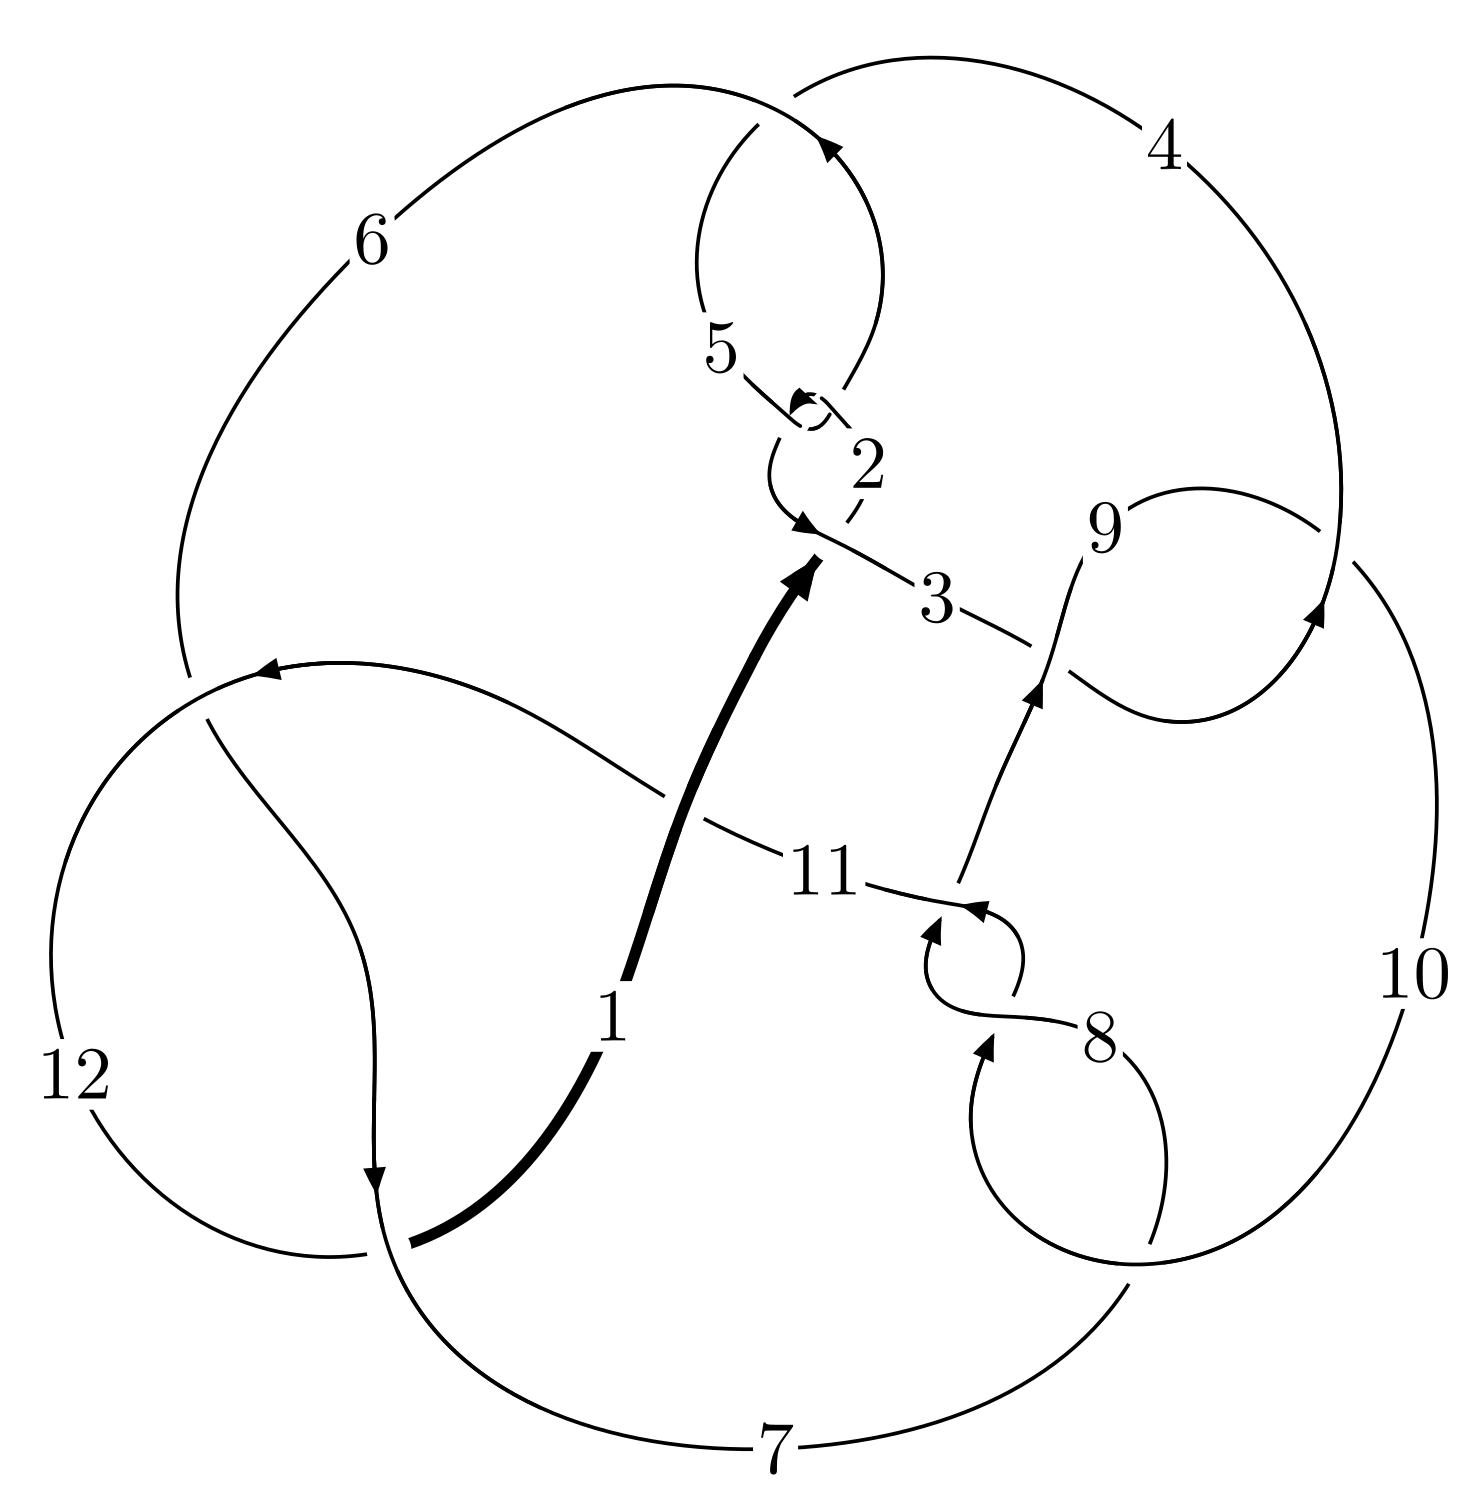
\includegraphics[width=112pt]{../../../GIT/diagram.site/Diagrams/png/983_12a_0182.png}\\
\ \ \ A knot diagram\footnotemark}&
\allowdisplaybreaks
\textbf{Linearized knot diagam} \\
\cline{2-2}
 &
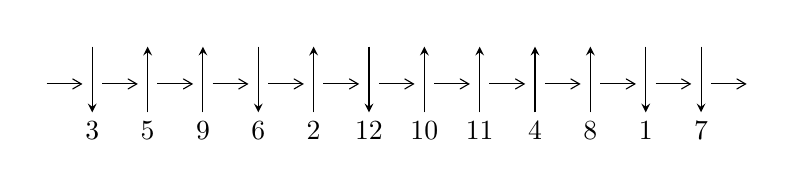
\begin{tikzpicture}[x=20pt, y=17pt]
	% nodes
	\node (C0) at (0, 0) {};
	\node (C1) at (1, 0) {};
	\node (C1U) at (1, +1) {};
	\node (C1D) at (1, -1) {3};

	\node (C2) at (2, 0) {};
	\node (C2U) at (2, +1) {};
	\node (C2D) at (2, -1) {5};

	\node (C3) at (3, 0) {};
	\node (C3U) at (3, +1) {};
	\node (C3D) at (3, -1) {9};

	\node (C4) at (4, 0) {};
	\node (C4U) at (4, +1) {};
	\node (C4D) at (4, -1) {6};

	\node (C5) at (5, 0) {};
	\node (C5U) at (5, +1) {};
	\node (C5D) at (5, -1) {2};

	\node (C6) at (6, 0) {};
	\node (C6U) at (6, +1) {};
	\node (C6D) at (6, -1) {12};

	\node (C7) at (7, 0) {};
	\node (C7U) at (7, +1) {};
	\node (C7D) at (7, -1) {10};

	\node (C8) at (8, 0) {};
	\node (C8U) at (8, +1) {};
	\node (C8D) at (8, -1) {11};

	\node (C9) at (9, 0) {};
	\node (C9U) at (9, +1) {};
	\node (C9D) at (9, -1) {4};

	\node (C10) at (10, 0) {};
	\node (C10U) at (10, +1) {};
	\node (C10D) at (10, -1) {8};

	\node (C11) at (11, 0) {};
	\node (C11U) at (11, +1) {};
	\node (C11D) at (11, -1) {1};

	\node (C12) at (12, 0) {};
	\node (C12U) at (12, +1) {};
	\node (C12D) at (12, -1) {7};
	\node (C13) at (13, 0) {};

	% arrows
	\draw[->,>={angle 60}]
	(C0) edge (C1) (C1) edge (C2) (C2) edge (C3) (C3) edge (C4) (C4) edge (C5) (C5) edge (C6) (C6) edge (C7) (C7) edge (C8) (C8) edge (C9) (C9) edge (C10) (C10) edge (C11) (C11) edge (C12) (C12) edge (C13) ;	\draw[->,>=stealth]
	(C1U) edge (C1D) (C2D) edge (C2U) (C3D) edge (C3U) (C4U) edge (C4D) (C5D) edge (C5U) (C6U) edge (C6D) (C7D) edge (C7U) (C8D) edge (C8U) (C9D) edge (C9U) (C10D) edge (C10U) (C11U) edge (C11D) (C12U) edge (C12D) ;
	\end{tikzpicture} \\
\hhline{~~} \\& 
\textbf{Solving Sequence} \\ \cline{2-2} 
 &
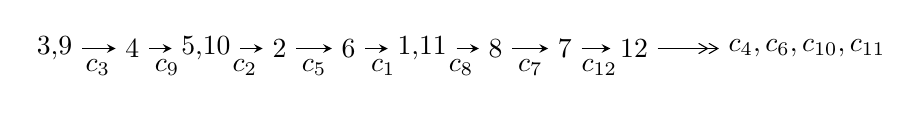
\begin{tikzpicture}[x=25pt, y=7pt]
	% node
	\node (A0) at (-1/8, 0) {3,9};
	\node (A1) at (1, 0) {4};
	\node (A2) at (33/16, 0) {5,10};
	\node (A3) at (25/8, 0) {2};
	\node (A4) at (33/8, 0) {6};
	\node (A5) at (83/16, 0) {1,11};
	\node (A6) at (25/4, 0) {8};
	\node (A7) at (29/4, 0) {7};
	\node (A8) at (33/4, 0) {12};
	\node (C1) at (1/2, -1) {$c_{3}$};
	\node (C2) at (3/2, -1) {$c_{9}$};
	\node (C3) at (21/8, -1) {$c_{2}$};
	\node (C4) at (29/8, -1) {$c_{5}$};
	\node (C5) at (37/8, -1) {$c_{1}$};
	\node (C6) at (23/4, -1) {$c_{8}$};
	\node (C7) at (27/4, -1) {$c_{7}$};
	\node (C8) at (31/4, -1) {$c_{12}$};
	\node (A9) at (43/4, 0) {$c_{4},c_{6},c_{10},c_{11}$};

	% edge
	\draw[->,>=stealth]	
	(A0) edge (A1) (A1) edge (A2) (A2) edge (A3) (A3) edge (A4) (A4) edge (A5) (A5) edge (A6) (A6) edge (A7) (A7) edge (A8) ;
	\draw[->>,>={angle 60}]	
	(A8) edge (A9);
\end{tikzpicture} \\ 

\end{tabular} \\

\footnotetext{
The image of knot diagram is generated by the software ``\textbf{Draw programme}" developed by Andrew Bartholomew(\url{http://www.layer8.co.uk/maths/draw/index.htm\#Running-draw}), where we modified some parts for our purpose(\url{https://github.com/CATsTAILs/LinksPainter}).
}\phantom \\ \newline 
\centering \textbf{Ideals for irreducible components\footnotemark of $X_{\text{par}}$} 
 
\begin{align*}
I^u_{1}&=\langle 
1.01638\times10^{144} u^{70}+3.79783\times10^{144} u^{69}+\cdots+2.19432\times10^{148} d+4.74337\times10^{147},\\
\phantom{I^u_{1}}&\phantom{= \langle  }-1.52787\times10^{144} u^{70}+2.07626\times10^{144} u^{69}+\cdots+3.13474\times10^{147} c-1.26268\times10^{147},\\
\phantom{I^u_{1}}&\phantom{= \langle  }2.08280\times10^{163} u^{70}-6.54445\times10^{163} u^{69}+\cdots+3.56067\times10^{166} b-1.75912\times10^{166},\\
\phantom{I^u_{1}}&\phantom{= \langle  }2.20933\times10^{163} u^{70}-4.97335\times10^{163} u^{69}+\cdots+1.01733\times10^{166} a-9.57968\times10^{164},\\
\phantom{I^u_{1}}&\phantom{= \langle  }u^{71}-2 u^{70}+\cdots+1536 u^2-512\rangle \\
I^u_{2}&=\langle 
c^2 u+u^2 c+d- c,\\
\phantom{I^u_{2}}&\phantom{= \langle  }u^8 c+u^8-3 u^6 c+u^7- u^5 c-2 u^6+4 u^4 c-3 u^5+2 u^3 c+u^4+c^3- u^2 c+3 u^3-2 c u+2 u^2- c-1,\\
\phantom{I^u_{2}}&\phantom{= \langle  }u^8-2 u^6+2 u^4+b,\;- u^6+u^4+a-1,\;u^9+u^8-2 u^7-3 u^6+u^5+3 u^4+2 u^3- u-1\rangle \\
\\
I^v_{1}&=\langle 
a,\;d- v+1,\;a v+c- v,\;b+v,\;v^2- v+1\rangle \\
I^v_{2}&=\langle 
a,\;d,\;c- v,\;b- v,\;v^2+v+1\rangle \\
I^v_{3}&=\langle 
c,\;d+1,\;b,\;a-1,\;v-1\rangle \\
I^v_{4}&=\langle 
a,\;d a- c b- d- b-1,\;d v+1,\;c v- b a- b v+b- a+1,\;b^2+b+1\rangle \\
\end{align*}
\raggedright * 5 irreducible components of $\dim_{\mathbb{C}}=0$, with total 103 representations.\\
\raggedright * 1 irreducible components of $\dim_{\mathbb{C}}=1$ \\
\footnotetext{All coefficients of polynomials are rational numbers. But the coefficients are sometimes approximated in decimal forms when there is not enough margin.}
\newpage
\renewcommand{\arraystretch}{1}
\centering \section*{I. $I^u_{1}= \langle 1.02\times10^{144} u^{70}+3.80\times10^{144} u^{69}+\cdots+2.19\times10^{148} d+4.74\times10^{147},\;-1.53\times10^{144} u^{70}+2.08\times10^{144} u^{69}+\cdots+3.13\times10^{147} c-1.26\times10^{147},\;2.08\times10^{163} u^{70}-6.54\times10^{163} u^{69}+\cdots+3.56\times10^{166} b-1.76\times10^{166},\;2.21\times10^{163} u^{70}-4.97\times10^{163} u^{69}+\cdots+1.02\times10^{166} a-9.58\times10^{164},\;u^{71}-2 u^{70}+\cdots+1536 u^2-512 \rangle$}
\flushleft \textbf{(i) Arc colorings}\\
\begin{tabular}{m{7pt} m{180pt} m{7pt} m{180pt} }
\flushright $a_{3}=$&$\begin{pmatrix}1\\0\end{pmatrix}$ \\
\flushright $a_{9}=$&$\begin{pmatrix}0\\u\end{pmatrix}$ \\
\flushright $a_{4}=$&$\begin{pmatrix}1\\- u^2\end{pmatrix}$ \\
\flushright $a_{5}=$&$\begin{pmatrix}-0.00217169 u^{70}+0.00488861 u^{69}+\cdots-2.25991 u+0.0941645\\-0.000584947 u^{70}+0.00183798 u^{69}+\cdots-0.979894 u+0.494041\end{pmatrix}$ \\
\flushright $a_{10}=$&$\begin{pmatrix}u\\- u^3+u\end{pmatrix}$ \\
\flushright $a_{2}=$&$\begin{pmatrix}0.000125704 u^{70}+0.00219339 u^{69}+\cdots-0.129419 u+0.703347\\0.000888998 u^{70}-0.00320644 u^{69}+\cdots+2.30414 u-0.769289\end{pmatrix}$ \\
\flushright $a_{6}=$&$\begin{pmatrix}0.000125704 u^{70}+0.00219339 u^{69}+\cdots-0.129419 u+0.703347\\-0.00231995 u^{70}+0.00405624 u^{69}+\cdots-2.36850 u-0.482448\end{pmatrix}$ \\
\flushright $a_{1}=$&$\begin{pmatrix}0.00101470 u^{70}-0.00101305 u^{69}+\cdots+2.17472 u-0.0659421\\0.000888998 u^{70}-0.00320644 u^{69}+\cdots+2.30414 u-0.769289\end{pmatrix}$ \\
\flushright $a_{11}=$&$\begin{pmatrix}0.000487399 u^{70}-0.000662337 u^{69}+\cdots+1.64247 u+0.402802\\-0.0000463186 u^{70}-0.000173075 u^{69}+\cdots+0.648446 u-0.216166\end{pmatrix}$ \\
\flushright $a_{8}=$&$\begin{pmatrix}-0.000515659 u^{70}+0.000632921 u^{69}+\cdots-0.744479 u-0.458988\\0.0000317918 u^{70}+0.0000611450 u^{69}+\cdots+1.16201 u+0.147793\end{pmatrix}$ \\
\flushright $a_{7}=$&$\begin{pmatrix}-0.000533717 u^{70}+0.000489262 u^{69}+\cdots-0.994027 u-0.618968\\0.000164426 u^{70}-0.000246208 u^{69}+\cdots+0.921710 u+0.0798584\end{pmatrix}$ \\
\flushright $a_{12}=$&$\begin{pmatrix}0.00194846 u^{70}-0.00138153 u^{69}+\cdots+2.53194 u+0.453579\\0.000595399 u^{70}-0.00245201 u^{69}+\cdots+1.96648 u-0.834037\end{pmatrix}$\\&\end{tabular}
\flushleft \textbf{(ii) Obstruction class $= -1$}\\~\\
\flushleft \textbf{(iii) Cusp Shapes $= 0.000644196 u^{70}+0.0111115 u^{69}+\cdots-0.863041 u+15.1191$}\\~\\
\newpage\renewcommand{\arraystretch}{1}
\flushleft \textbf{(iv) u-Polynomials at the component}\newline \\
\begin{tabular}{m{50pt}|m{274pt}}
Crossings & \hspace{64pt}u-Polynomials at each crossing \\
\hline $$\begin{aligned}c_{1},c_{4}\end{aligned}$$&$\begin{aligned}
&u^{71}+24 u^{70}+\cdots-40 u-16
\end{aligned}$\\
\hline $$\begin{aligned}c_{2},c_{5}\end{aligned}$$&$\begin{aligned}
&u^{71}+2 u^{70}+\cdots-5 u^2-4
\end{aligned}$\\
\hline $$\begin{aligned}c_{3},c_{9}\end{aligned}$$&$\begin{aligned}
&u^{71}-2 u^{70}+\cdots+1536 u^2-512
\end{aligned}$\\
\hline $$\begin{aligned}c_{6},c_{12}\end{aligned}$$&$\begin{aligned}
&u^{71}-8 u^{70}+\cdots+56 u-16
\end{aligned}$\\
\hline $$\begin{aligned}c_{7},c_{8},c_{10}\end{aligned}$$&$\begin{aligned}
&u^{71}+8 u^{70}+\cdots+56 u-16
\end{aligned}$\\
\hline $$\begin{aligned}c_{11}\end{aligned}$$&$\begin{aligned}
&u^{71}+30 u^{70}+\cdots+4640 u+256
\end{aligned}$\\
\hline
\end{tabular}\\~\\
\newpage\renewcommand{\arraystretch}{1}
\flushleft \textbf{(v) Riley Polynomials at the component}\newline \\
\begin{tabular}{m{50pt}|m{274pt}}
Crossings & \hspace{64pt}Riley Polynomials at each crossing \\
\hline $$\begin{aligned}c_{1},c_{4}\end{aligned}$$&$\begin{aligned}
&y^{71}+48 y^{70}+\cdots-6880 y-256
\end{aligned}$\\
\hline $$\begin{aligned}c_{2},c_{5}\end{aligned}$$&$\begin{aligned}
&y^{71}+24 y^{70}+\cdots-40 y-16
\end{aligned}$\\
\hline $$\begin{aligned}c_{3},c_{9}\end{aligned}$$&$\begin{aligned}
&y^{71}-30 y^{70}+\cdots+1572864 y-262144
\end{aligned}$\\
\hline $$\begin{aligned}c_{6},c_{12}\end{aligned}$$&$\begin{aligned}
&y^{71}-30 y^{70}+\cdots+4640 y-256
\end{aligned}$\\
\hline $$\begin{aligned}c_{7},c_{8},c_{10}\end{aligned}$$&$\begin{aligned}
&y^{71}-70 y^{70}+\cdots-1504 y-256
\end{aligned}$\\
\hline $$\begin{aligned}c_{11}\end{aligned}$$&$\begin{aligned}
&y^{71}+30 y^{70}+\cdots+5022208 y-65536
\end{aligned}$\\
\hline
\end{tabular}\\~\\
\newpage\flushleft \textbf{(vi) Complex Volumes and Cusp Shapes}
$$\begin{array}{c|c|c}  
\text{Solutions to }I^u_{1}& \I (\text{vol} + \sqrt{-1}CS) & \text{Cusp shape}\\
 \hline 
\begin{aligned}
u &= -0.372595 + 0.922213 I \\
a &= \phantom{-}0.706869 + 0.294839 I \\
b &= -0.705480 + 0.710846 I \\
c &= -0.470907 + 0.554383 I \\
d &= -1.70042 + 0.50968 I\end{aligned}
 & -0.206074 + 1.106620 I & \phantom{-}1.82615 - 2.10157 I \\ \hline\begin{aligned}
u &= -0.372595 - 0.922213 I \\
a &= \phantom{-}0.706869 - 0.294839 I \\
b &= -0.705480 - 0.710846 I \\
c &= -0.470907 - 0.554383 I \\
d &= -1.70042 - 0.50968 I\end{aligned}
 & -0.206074 - 1.106620 I & \phantom{-}1.82615 + 2.10157 I \\ \hline\begin{aligned}
u &= \phantom{-}0.661751 + 0.731261 I \\
a &= \phantom{-}1.05387 - 1.06299 I \\
b &= \phantom{-}0.033676 - 0.991675 I \\
c &= \phantom{-}0.475791 + 0.487011 I \\
d &= \phantom{-}1.339240 - 0.225092 I\end{aligned}
 & -5.31233 - 1.23150 I & -6.16629 + 0.79467 I \\ \hline\begin{aligned}
u &= \phantom{-}0.661751 - 0.731261 I \\
a &= \phantom{-}1.05387 + 1.06299 I \\
b &= \phantom{-}0.033676 + 0.991675 I \\
c &= \phantom{-}0.475791 - 0.487011 I \\
d &= \phantom{-}1.339240 + 0.225092 I\end{aligned}
 & -5.31233 + 1.23150 I & -6.16629 - 0.79467 I \\ \hline\begin{aligned}
u &= \phantom{-}0.216094 + 0.961248 I \\
a &= \phantom{-}0.490833 + 0.220678 I \\
b &= \phantom{-}0.626372 - 0.146182 I \\
c &= \phantom{-}0.190153 - 1.314880 I \\
d &= -0.304165 - 0.812210 I\end{aligned}
 & \phantom{-}2.60149 - 2.06138 I & \phantom{-}6.60052 + 3.22142 I \\ \hline\begin{aligned}
u &= \phantom{-}0.216094 - 0.961248 I \\
a &= \phantom{-}0.490833 - 0.220678 I \\
b &= \phantom{-}0.626372 + 0.146182 I \\
c &= \phantom{-}0.190153 + 1.314880 I \\
d &= -0.304165 + 0.812210 I\end{aligned}
 & \phantom{-}2.60149 + 2.06138 I & \phantom{-}6.60052 - 3.22142 I\\
 \hline 
 \end{array}$$\newpage$$\begin{array}{c|c|c}  
\text{Solutions to }I^u_{1}& \I (\text{vol} + \sqrt{-1}CS) & \text{Cusp shape}\\
 \hline 
\begin{aligned}
u &= -0.510340 + 0.919175 I \\
a &= \phantom{-}0.97241 + 1.52837 I \\
b &= \phantom{-}0.167182 + 1.050320 I \\
c &= -0.387643 - 1.176070 I \\
d &= \phantom{-}0.698084 - 0.628537 I\end{aligned}
 & -1.22762 + 4.53498 I & -0.48837 - 4.83158 I \\ \hline\begin{aligned}
u &= -0.510340 - 0.919175 I \\
a &= \phantom{-}0.97241 - 1.52837 I \\
b &= \phantom{-}0.167182 - 1.050320 I \\
c &= -0.387643 + 1.176070 I \\
d &= \phantom{-}0.698084 + 0.628537 I\end{aligned}
 & -1.22762 - 4.53498 I & -0.48837 + 4.83158 I \\ \hline\begin{aligned}
u &= \phantom{-}0.843761 + 0.417994 I \\
a &= -3.24462 + 0.27087 I \\
b &= \phantom{-}0.648309 + 0.950753 I \\
c &= \phantom{-}0.537281 + 0.453998 I \\
d &= \phantom{-}0.703145 - 0.615016 I\end{aligned}
 & -1.74336 + 3.95563 I & \phantom{-}0.57229 - 6.63484 I \\ \hline\begin{aligned}
u &= \phantom{-}0.843761 - 0.417994 I \\
a &= -3.24462 - 0.27087 I \\
b &= \phantom{-}0.648309 - 0.950753 I \\
c &= \phantom{-}0.537281 - 0.453998 I \\
d &= \phantom{-}0.703145 + 0.615016 I\end{aligned}
 & -1.74336 - 3.95563 I & \phantom{-}0.57229 + 6.63484 I \\ \hline\begin{aligned}
u &= -0.980094 + 0.401535 I \\
a &= \phantom{-}0.780465 + 0.104472 I \\
b &= -0.675884 + 0.258339 I \\
c &= -0.548184 + 0.485014 I \\
d &= -0.641289 - 0.881527 I\end{aligned}
 & \phantom{-}0.13020 - 4.00402 I & \phantom{-}4.41276 + 6.69495 I \\ \hline\begin{aligned}
u &= -0.980094 - 0.401535 I \\
a &= \phantom{-}0.780465 - 0.104472 I \\
b &= -0.675884 - 0.258339 I \\
c &= -0.548184 - 0.485014 I \\
d &= -0.641289 + 0.881527 I\end{aligned}
 & \phantom{-}0.13020 + 4.00402 I & \phantom{-}4.41276 - 6.69495 I\\
 \hline 
 \end{array}$$\newpage$$\begin{array}{c|c|c}  
\text{Solutions to }I^u_{1}& \I (\text{vol} + \sqrt{-1}CS) & \text{Cusp shape}\\
 \hline 
\begin{aligned}
u &= \phantom{-}0.482781 + 0.984718 I \\
a &= \phantom{-}0.632388 + 0.401253 I \\
b &= -0.681961 + 0.973056 I \\
c &= \phantom{-}0.486783 + 0.532736 I \\
d &= \phantom{-}1.88522 + 0.25805 I\end{aligned}
 & -0.99233 - 6.45679 I & \phantom{-}0.34368 + 6.97496 I \\ \hline\begin{aligned}
u &= \phantom{-}0.482781 - 0.984718 I \\
a &= \phantom{-}0.632388 - 0.401253 I \\
b &= -0.681961 - 0.973056 I \\
c &= \phantom{-}0.486783 - 0.532736 I \\
d &= \phantom{-}1.88522 - 0.25805 I\end{aligned}
 & -0.99233 + 6.45679 I & \phantom{-}0.34368 - 6.97496 I \\ \hline\begin{aligned}
u &= \phantom{-}0.777198 + 0.427799 I \\
a &= \phantom{-}0.661548 + 0.487935 I \\
b &= -0.527615 + 1.024960 I \\
c &= \phantom{-}0.525019 + 0.439223 I \\
d &= \phantom{-}0.729049 - 0.488658 I\end{aligned}
 & -1.94652 - 0.34051 I & -0.37051 - 3.03065 I \\ \hline\begin{aligned}
u &= \phantom{-}0.777198 - 0.427799 I \\
a &= \phantom{-}0.661548 - 0.487935 I \\
b &= -0.527615 - 1.024960 I \\
c &= \phantom{-}0.525019 - 0.439223 I \\
d &= \phantom{-}0.729049 + 0.488658 I\end{aligned}
 & -1.94652 + 0.34051 I & -0.37051 + 3.03065 I \\ \hline\begin{aligned}
u &= \phantom{-}1.127060 + 0.152551 I \\
a &= \phantom{-}0.639024 + 0.570894 I \\
b &= -0.435782 + 1.114890 I \\
c &= -1.214770 + 0.100113 I \\
d &= -1.35450 + 0.44354 I\end{aligned}
 & \phantom{-}4.50468 - 2.47836 I & \phantom{-}7.49354 + 3.38416 I \\ \hline\begin{aligned}
u &= \phantom{-}1.127060 - 0.152551 I \\
a &= \phantom{-}0.639024 - 0.570894 I \\
b &= -0.435782 - 1.114890 I \\
c &= -1.214770 - 0.100113 I \\
d &= -1.35450 - 0.44354 I\end{aligned}
 & \phantom{-}4.50468 + 2.47836 I & \phantom{-}7.49354 - 3.38416 I\\
 \hline 
 \end{array}$$\newpage$$\begin{array}{c|c|c}  
\text{Solutions to }I^u_{1}& \I (\text{vol} + \sqrt{-1}CS) & \text{Cusp shape}\\
 \hline 
\begin{aligned}
u &= \phantom{-}0.982347 + 0.611518 I \\
a &= \phantom{-}0.755795 - 0.846393 I \\
b &= -0.132131 - 1.098790 I \\
c &= \phantom{-}0.515465 + 0.490470 I \\
d &= \phantom{-}1.08458 - 0.93082 I\end{aligned}
 & -4.29573 + 6.37313 I & -3.00781 - 7.19219 I \\ \hline\begin{aligned}
u &= \phantom{-}0.982347 - 0.611518 I \\
a &= \phantom{-}0.755795 + 0.846393 I \\
b &= -0.132131 + 1.098790 I \\
c &= \phantom{-}0.515465 - 0.490470 I \\
d &= \phantom{-}1.08458 + 0.93082 I\end{aligned}
 & -4.29573 - 6.37313 I & -3.00781 + 7.19219 I \\ \hline\begin{aligned}
u &= \phantom{-}1.173990 + 0.222972 I \\
a &= -2.07252 - 0.44952 I \\
b &= \phantom{-}0.744384 + 0.914398 I \\
c &= \phantom{-}0.606381 - 0.672488 I \\
d &= -0.633879 + 0.879788 I\end{aligned}
 & \phantom{-}5.09577 + 1.83902 I & \phantom{-}8.24819 + 0. I\phantom{ +0.000000I} \\ \hline\begin{aligned}
u &= \phantom{-}1.173990 - 0.222972 I \\
a &= -2.07252 + 0.44952 I \\
b &= \phantom{-}0.744384 - 0.914398 I \\
c &= \phantom{-}0.606381 + 0.672488 I \\
d &= -0.633879 - 0.879788 I\end{aligned}
 & \phantom{-}5.09577 - 1.83902 I & \phantom{-}8.24819 + 0. I\phantom{ +0.000000I} \\ \hline\begin{aligned}
u &= -1.203430 + 0.094057 I \\
a &= -1.52309 - 0.96637 I \\
b &= \phantom{-}0.774513 + 0.827694 I \\
c &= -0.596615 - 0.625599 I \\
d &= \phantom{-}0.431350 + 1.041490 I\end{aligned}
 & \phantom{-}5.36659 + 3.89584 I & \phantom{-}8.41567 - 5.55146 I \\ \hline\begin{aligned}
u &= -1.203430 - 0.094057 I \\
a &= -1.52309 + 0.96637 I \\
b &= \phantom{-}0.774513 - 0.827694 I \\
c &= -0.596615 + 0.625599 I \\
d &= \phantom{-}0.431350 - 1.041490 I\end{aligned}
 & \phantom{-}5.36659 - 3.89584 I & \phantom{-}8.41567 + 5.55146 I\\
 \hline 
 \end{array}$$\newpage$$\begin{array}{c|c|c}  
\text{Solutions to }I^u_{1}& \I (\text{vol} + \sqrt{-1}CS) & \text{Cusp shape}\\
 \hline 
\begin{aligned}
u &= \phantom{-}1.117530 + 0.478181 I \\
a &= \phantom{-}0.690211 - 0.765567 I \\
b &= -0.209298 - 1.133130 I \\
c &= -1.116800 + 0.271956 I \\
d &= -1.28841 + 1.30589 I\end{aligned}
 & \phantom{-}3.15531 + 5.12152 I & \phantom{-0.000000 } 0 \\ \hline\begin{aligned}
u &= \phantom{-}1.117530 - 0.478181 I \\
a &= \phantom{-}0.690211 + 0.765567 I \\
b &= -0.209298 + 1.133130 I \\
c &= -1.116800 - 0.271956 I \\
d &= -1.28841 - 1.30589 I\end{aligned}
 & \phantom{-}3.15531 - 5.12152 I & \phantom{-0.000000 } 0 \\ \hline\begin{aligned}
u &= -1.137650 + 0.460214 I \\
a &= \phantom{-}0.609632 - 0.520416 I \\
b &= -0.523715 - 1.123490 I \\
c &= \phantom{-}1.116170 + 0.256986 I \\
d &= \phantom{-}1.24509 + 1.25727 I\end{aligned}
 & \phantom{-}3.19656 - 2.55854 I & \phantom{-0.000000 } 0 \\ \hline\begin{aligned}
u &= -1.137650 - 0.460214 I \\
a &= \phantom{-}0.609632 + 0.520416 I \\
b &= -0.523715 + 1.123490 I \\
c &= \phantom{-}1.116170 - 0.256986 I \\
d &= \phantom{-}1.24509 - 1.25727 I\end{aligned}
 & \phantom{-}3.19656 + 2.55854 I & \phantom{-0.000000 } 0 \\ \hline\begin{aligned}
u &= -0.725491 + 0.260568 I \\
a &= -0.74999 - 2.93714 I \\
b &= \phantom{-}0.621787 + 0.746410 I \\
c &= -0.573783 + 0.383951 I \\
d &= -0.438809 - 0.376035 I\end{aligned}
 & -1.09934 + 1.05821 I & \phantom{-}3.09814 + 1.72718 I \\ \hline\begin{aligned}
u &= -0.725491 - 0.260568 I \\
a &= -0.74999 + 2.93714 I \\
b &= \phantom{-}0.621787 - 0.746410 I \\
c &= -0.573783 - 0.383951 I \\
d &= -0.438809 + 0.376035 I\end{aligned}
 & -1.09934 - 1.05821 I & \phantom{-}3.09814 - 1.72718 I\\
 \hline 
 \end{array}$$\newpage$$\begin{array}{c|c|c}  
\text{Solutions to }I^u_{1}& \I (\text{vol} + \sqrt{-1}CS) & \text{Cusp shape}\\
 \hline 
\begin{aligned}
u &= -0.247645 + 1.226350 I \\
a &= \phantom{-}0.653789 + 0.300056 I \\
b &= -0.795711 + 0.784067 I \\
c &= -0.133830 - 1.140380 I \\
d &= \phantom{-}0.422479 - 1.218340 I\end{aligned}
 & \phantom{-}6.94619 - 1.12108 I & \phantom{-0.000000 } 0 \\ \hline\begin{aligned}
u &= -0.247645 - 1.226350 I \\
a &= \phantom{-}0.653789 - 0.300056 I \\
b &= -0.795711 - 0.784067 I \\
c &= -0.133830 + 1.140380 I \\
d &= \phantom{-}0.422479 + 1.218340 I\end{aligned}
 & \phantom{-}6.94619 + 1.12108 I & \phantom{-0.000000 } 0 \\ \hline\begin{aligned}
u &= \phantom{-}0.464983 + 0.581438 I \\
a &= \phantom{-}1.72522 - 0.64973 I \\
b &= \phantom{-}0.139048 - 0.768176 I \\
c &= \phantom{-}0.71852 - 1.33569 I \\
d &= -0.442687 - 0.257326 I\end{aligned}
 & \phantom{-}1.011140 - 0.938516 I & \phantom{-}3.66296 - 0.79830 I \\ \hline\begin{aligned}
u &= \phantom{-}0.464983 - 0.581438 I \\
a &= \phantom{-}1.72522 + 0.64973 I \\
b &= \phantom{-}0.139048 + 0.768176 I \\
c &= \phantom{-}0.71852 + 1.33569 I \\
d &= -0.442687 + 0.257326 I\end{aligned}
 & \phantom{-}1.011140 + 0.938516 I & \phantom{-}3.66296 + 0.79830 I \\ \hline\begin{aligned}
u &= \phantom{-}0.368570 + 1.210560 I \\
a &= \phantom{-}0.618935 + 0.372180 I \\
b &= -0.745652 + 0.954700 I \\
c &= \phantom{-}0.194177 - 1.117100 I \\
d &= -0.623618 - 1.150760 I\end{aligned}
 & \phantom{-}6.42018 - 4.68044 I & \phantom{-0.000000 } 0 \\ \hline\begin{aligned}
u &= \phantom{-}0.368570 - 1.210560 I \\
a &= \phantom{-}0.618935 - 0.372180 I \\
b &= -0.745652 - 0.954700 I \\
c &= \phantom{-}0.194177 + 1.117100 I \\
d &= -0.623618 + 1.150760 I\end{aligned}
 & \phantom{-}6.42018 + 4.68044 I & \phantom{-0.000000 } 0\\
 \hline 
 \end{array}$$\newpage$$\begin{array}{c|c|c}  
\text{Solutions to }I^u_{1}& \I (\text{vol} + \sqrt{-1}CS) & \text{Cusp shape}\\
 \hline 
\begin{aligned}
u &= -1.248660 + 0.306382 I \\
a &= \phantom{-}0.734113 + 0.059783 I \\
b &= -0.802776 + 0.158635 I \\
c &= \phantom{-}1.116690 + 0.156605 I \\
d &= \phantom{-}0.994223 + 0.843737 I\end{aligned}
 & \phantom{-}7.51654 - 1.91781 I & \phantom{-0.000000 } 0 \\ \hline\begin{aligned}
u &= -1.248660 - 0.306382 I \\
a &= \phantom{-}0.734113 - 0.059783 I \\
b &= -0.802776 - 0.158635 I \\
c &= \phantom{-}1.116690 - 0.156605 I \\
d &= \phantom{-}0.994223 - 0.843737 I\end{aligned}
 & \phantom{-}7.51654 + 1.91781 I & \phantom{-0.000000 } 0 \\ \hline\begin{aligned}
u &= \phantom{-}0.504947 + 1.215580 I \\
a &= \phantom{-}0.662564 - 0.264148 I \\
b &= -0.825179 - 0.702952 I \\
c &= \phantom{-}0.245007 - 1.071700 I \\
d &= -0.859773 - 1.094450 I\end{aligned}
 & \phantom{-}5.42990 - 4.32973 I & \phantom{-0.000000 } 0 \\ \hline\begin{aligned}
u &= \phantom{-}0.504947 - 1.215580 I \\
a &= \phantom{-}0.662564 + 0.264148 I \\
b &= -0.825179 + 0.702952 I \\
c &= \phantom{-}0.245007 + 1.071700 I \\
d &= -0.859773 + 1.094450 I\end{aligned}
 & \phantom{-}5.42990 + 4.32973 I & \phantom{-0.000000 } 0 \\ \hline\begin{aligned}
u &= -1.152900 + 0.667545 I \\
a &= \phantom{-}0.653927 + 0.849988 I \\
b &= -0.143613 + 1.176100 I \\
c &= \phantom{-}1.028980 + 0.314229 I \\
d &= \phantom{-}1.17468 + 1.72508 I\end{aligned}
 & \phantom{-}0.80414 - 10.42400 I & \phantom{-0.000000 } 0 \\ \hline\begin{aligned}
u &= -1.152900 - 0.667545 I \\
a &= \phantom{-}0.653927 - 0.849988 I \\
b &= -0.143613 - 1.176100 I \\
c &= \phantom{-}1.028980 - 0.314229 I \\
d &= \phantom{-}1.17468 - 1.72508 I\end{aligned}
 & \phantom{-}0.80414 + 10.42400 I & \phantom{-0.000000 } 0\\
 \hline 
 \end{array}$$\newpage$$\begin{array}{c|c|c}  
\text{Solutions to }I^u_{1}& \I (\text{vol} + \sqrt{-1}CS) & \text{Cusp shape}\\
 \hline 
\begin{aligned}
u &= -1.185800 + 0.609579 I \\
a &= -0.604647 - 0.948689 I \\
b &= \phantom{-}0.833000 + 0.664986 I \\
c &= -0.515530 + 0.509861 I \\
d &= -1.03285 - 1.38981 I\end{aligned}
 & \phantom{-}2.33908 - 6.73341 I & \phantom{-0.000000 } 0 \\ \hline\begin{aligned}
u &= -1.185800 - 0.609579 I \\
a &= -0.604647 + 0.948689 I \\
b &= \phantom{-}0.833000 - 0.664986 I \\
c &= -0.515530 - 0.509861 I \\
d &= -1.03285 + 1.38981 I\end{aligned}
 & \phantom{-}2.33908 + 6.73341 I & \phantom{-0.000000 } 0 \\ \hline\begin{aligned}
u &= -0.593784 + 1.208600 I \\
a &= \phantom{-}0.602225 - 0.393473 I \\
b &= -0.733361 - 1.011480 I \\
c &= -0.274626 - 1.042820 I \\
d &= \phantom{-}1.00911 - 1.02929 I\end{aligned}
 & \phantom{-}4.48821 + 10.17210 I & \phantom{-0.000000 } 0 \\ \hline\begin{aligned}
u &= -0.593784 - 1.208600 I \\
a &= \phantom{-}0.602225 + 0.393473 I \\
b &= -0.733361 + 1.011480 I \\
c &= -0.274626 + 1.042820 I \\
d &= \phantom{-}1.00911 + 1.02929 I\end{aligned}
 & \phantom{-}4.48821 - 10.17210 I & \phantom{-0.000000 } 0 \\ \hline\begin{aligned}
u &= \phantom{-}1.233000 + 0.545251 I \\
a &= \phantom{-}0.716779 - 0.101507 I \\
b &= -0.834377 - 0.273084 I \\
c &= -1.052540 + 0.252051 I \\
d &= -1.00331 + 1.44383 I\end{aligned}
 & \phantom{-}5.82408 + 7.48275 I & \phantom{-0.000000 } 0 \\ \hline\begin{aligned}
u &= \phantom{-}1.233000 - 0.545251 I \\
a &= \phantom{-}0.716779 + 0.101507 I \\
b &= -0.834377 + 0.273084 I \\
c &= -1.052540 - 0.252051 I \\
d &= -1.00331 - 1.44383 I\end{aligned}
 & \phantom{-}5.82408 - 7.48275 I & \phantom{-0.000000 } 0\\
 \hline 
 \end{array}$$\newpage$$\begin{array}{c|c|c}  
\text{Solutions to }I^u_{1}& \I (\text{vol} + \sqrt{-1}CS) & \text{Cusp shape}\\
 \hline 
\begin{aligned}
u &= -0.176438 + 0.617781 I \\
a &= -1.24181 - 5.67569 I \\
b &= \phantom{-}0.472468 - 0.965679 I \\
c &= -0.38103 - 1.75179 I \\
d &= \phantom{-}0.176185 - 0.407221 I\end{aligned}
 & \phantom{-}0.42738 - 1.60074 I & \phantom{-}0.77404 + 2.18898 I \\ \hline\begin{aligned}
u &= -0.176438 - 0.617781 I \\
a &= -1.24181 + 5.67569 I \\
b &= \phantom{-}0.472468 + 0.965679 I \\
c &= -0.38103 + 1.75179 I \\
d &= \phantom{-}0.176185 + 0.407221 I\end{aligned}
 & \phantom{-}0.42738 + 1.60074 I & \phantom{-}0.77404 - 2.18898 I \\ \hline\begin{aligned}
u &= \phantom{-}1.181300 + 0.680585 I \\
a &= -1.94797 + 0.51901 I \\
b &= \phantom{-}0.722487 + 1.031630 I \\
c &= \phantom{-}0.510240 + 0.507622 I \\
d &= \phantom{-}1.20020 - 1.39980 I\end{aligned}
 & \phantom{-}1.22414 + 12.55690 I & \phantom{-0.000000 } 0 \\ \hline\begin{aligned}
u &= \phantom{-}1.181300 - 0.680585 I \\
a &= -1.94797 - 0.51901 I \\
b &= \phantom{-}0.722487 - 1.031630 I \\
c &= \phantom{-}0.510240 - 0.507622 I \\
d &= \phantom{-}1.20020 + 1.39980 I\end{aligned}
 & \phantom{-}1.22414 - 12.55690 I & \phantom{-0.000000 } 0 \\ \hline\begin{aligned}
u &= \phantom{-}0.010891 + 0.626888 I \\
a &= \phantom{-}0.717451 - 0.379980 I \\
b &= -0.596253 - 0.833536 I \\
c &= -0.145864 + 0.996178 I \\
d &= -0.36117 + 2.00147 I\end{aligned}
 & \phantom{-}0.65592 + 2.35939 I & \phantom{-}1.51759 - 4.85897 I \\ \hline\begin{aligned}
u &= \phantom{-}0.010891 - 0.626888 I \\
a &= \phantom{-}0.717451 + 0.379980 I \\
b &= -0.596253 + 0.833536 I \\
c &= -0.145864 - 0.996178 I \\
d &= -0.36117 - 2.00147 I\end{aligned}
 & \phantom{-}0.65592 - 2.35939 I & \phantom{-}1.51759 + 4.85897 I\\
 \hline 
 \end{array}$$\newpage$$\begin{array}{c|c|c}  
\text{Solutions to }I^u_{1}& \I (\text{vol} + \sqrt{-1}CS) & \text{Cusp shape}\\
 \hline 
\begin{aligned}
u &= -0.617428 + 0.085193 I \\
a &= \phantom{-}0.771703 + 0.515946 I \\
b &= -0.399151 + 0.927946 I \\
c &= -0.667996 + 0.208298 I \\
d &= -0.215095 - 0.146010 I\end{aligned}
 & -0.93328 - 2.67780 I & \phantom{-}3.99337 + 7.95500 I \\ \hline\begin{aligned}
u &= -0.617428 - 0.085193 I \\
a &= \phantom{-}0.771703 - 0.515946 I \\
b &= -0.399151 - 0.927946 I \\
c &= -0.667996 - 0.208298 I \\
d &= -0.215095 + 0.146010 I\end{aligned}
 & -0.93328 + 2.67780 I & \phantom{-}3.99337 - 7.95500 I \\ \hline\begin{aligned}
u &= \phantom{-}0.591164\phantom{ +0.000000I} \\
a &= \phantom{-}0.929806\phantom{ +0.000000I} \\
b &= -0.315087\phantom{ +0.000000I} \\
c &= \phantom{-}1.20948\phantom{ +0.000000I} \\
d &= -0.0779789\phantom{ +0.000000I}\end{aligned}
 & \phantom{-}1.02886\phantom{ +0.000000I} & \phantom{-}10.5160\phantom{ +0.000000I} \\ \hline\begin{aligned}
u &= -0.282782 + 0.492299 I \\
a &= \phantom{-}1.070690 - 0.124673 I \\
b &= \phantom{-}0.198227 + 0.270585 I \\
c &= -0.298696 + 0.445240 I \\
d &= -0.632940 + 0.412834 I\end{aligned}
 & -1.67984 + 0.60130 I & -3.90300 - 0.33160 I \\ \hline\begin{aligned}
u &= -0.282782 - 0.492299 I \\
a &= \phantom{-}1.070690 + 0.124673 I \\
b &= \phantom{-}0.198227 - 0.270585 I \\
c &= -0.298696 - 0.445240 I \\
d &= -0.632940 - 0.412834 I\end{aligned}
 & -1.67984 - 0.60130 I & -3.90300 + 0.33160 I \\ \hline\begin{aligned}
u &= -1.33133 + 0.61244 I \\
a &= -0.691353 - 0.789833 I \\
b &= \phantom{-}0.877454 + 0.689350 I \\
c &= \phantom{-}1.004370 + 0.240216 I \\
d &= \phantom{-}0.77088 + 1.60236 I\end{aligned}
 & \phantom{-}10.54930 - 5.35435 I & \phantom{-0.000000 } 0\\
 \hline 
 \end{array}$$\newpage$$\begin{array}{c|c|c}  
\text{Solutions to }I^u_{1}& \I (\text{vol} + \sqrt{-1}CS) & \text{Cusp shape}\\
 \hline 
\begin{aligned}
u &= -1.33133 - 0.61244 I \\
a &= -0.691353 + 0.789833 I \\
b &= \phantom{-}0.877454 - 0.689350 I \\
c &= \phantom{-}1.004370 - 0.240216 I \\
d &= \phantom{-}0.77088 - 1.60236 I\end{aligned}
 & \phantom{-}10.54930 + 5.35435 I & \phantom{-0.000000 } 0 \\ \hline\begin{aligned}
u &= \phantom{-}1.29995 + 0.68416 I \\
a &= -1.77475 + 0.42337 I \\
b &= \phantom{-}0.751329 + 1.038160 I \\
c &= -0.990397 + 0.266490 I \\
d &= -0.85024 + 1.76626 I\end{aligned}
 & \phantom{-}9.4739 + 11.4004 I & \phantom{-0.000000 } 0 \\ \hline\begin{aligned}
u &= \phantom{-}1.29995 - 0.68416 I \\
a &= -1.77475 - 0.42337 I \\
b &= \phantom{-}0.751329 - 1.038160 I \\
c &= -0.990397 - 0.266490 I \\
d &= -0.85024 - 1.76626 I\end{aligned}
 & \phantom{-}9.4739 - 11.4004 I & \phantom{-0.000000 } 0 \\ \hline\begin{aligned}
u &= \phantom{-}1.27239 + 0.75883 I \\
a &= -0.528127 + 0.758818 I \\
b &= \phantom{-}0.887462 - 0.636245 I \\
c &= -0.972392 + 0.290048 I \\
d &= -0.92205 + 1.92929 I\end{aligned}
 & \phantom{-}7.95427 + 11.37060 I & \phantom{-0.000000 } 0 \\ \hline\begin{aligned}
u &= \phantom{-}1.27239 - 0.75883 I \\
a &= -0.528127 - 0.758818 I \\
b &= \phantom{-}0.887462 + 0.636245 I \\
c &= -0.972392 - 0.290048 I \\
d &= -0.92205 - 1.92929 I\end{aligned}
 & \phantom{-}7.95427 - 11.37060 I & \phantom{-0.000000 } 0 \\ \hline\begin{aligned}
u &= -1.24401 + 0.80606 I \\
a &= -1.73933 - 0.62055 I \\
b &= \phantom{-}0.732124 - 1.065030 I \\
c &= \phantom{-}0.961782 + 0.307183 I \\
d &= \phantom{-}0.99186 + 2.02574 I\end{aligned}
 & \phantom{-}6.6365 - 17.3722 I & \phantom{-0.000000 } 0\\
 \hline 
 \end{array}$$\newpage$$\begin{array}{c|c|c}  
\text{Solutions to }I^u_{1}& \I (\text{vol} + \sqrt{-1}CS) & \text{Cusp shape}\\
 \hline 
\begin{aligned}
u &= -1.24401 - 0.80606 I \\
a &= -1.73933 + 0.62055 I \\
b &= \phantom{-}0.732124 + 1.065030 I \\
c &= \phantom{-}0.961782 - 0.307183 I \\
d &= \phantom{-}0.99186 - 2.02574 I\end{aligned}
 & \phantom{-}6.6365 + 17.3722 I & \phantom{-0.000000 } 0 \\ \hline\begin{aligned}
u &= -1.51788 + 0.06429 I \\
a &= -1.289590 - 0.499691 I \\
b &= \phantom{-}0.858480 + 0.864860 I \\
c &= \phantom{-}1.033780 + 0.023696 I \\
d &= \phantom{-}0.276083 + 0.176660 I\end{aligned}
 & \phantom{-}13.78050 - 0.08878 I & \phantom{-0.000000 } 0 \\ \hline\begin{aligned}
u &= -1.51788 - 0.06429 I \\
a &= -1.289590 + 0.499691 I \\
b &= \phantom{-}0.858480 - 0.864860 I \\
c &= \phantom{-}1.033780 - 0.023696 I \\
d &= \phantom{-}0.276083 - 0.176660 I\end{aligned}
 & \phantom{-}13.78050 + 0.08878 I & \phantom{-0.000000 } 0 \\ \hline\begin{aligned}
u &= \phantom{-}1.51414 + 0.16464 I \\
a &= -1.47755 - 0.28880 I \\
b &= \phantom{-}0.837181 + 0.923149 I \\
c &= -1.029750 + 0.060361 I \\
d &= -0.287259 + 0.451271 I\end{aligned}
 & \phantom{-}13.6007 + 6.3599 I & \phantom{-0.000000 } 0 \\ \hline\begin{aligned}
u &= \phantom{-}1.51414 - 0.16464 I \\
a &= -1.47755 + 0.28880 I \\
b &= \phantom{-}0.837181 - 0.923149 I \\
c &= -1.029750 - 0.060361 I \\
d &= -0.287259 - 0.451271 I\end{aligned}
 & \phantom{-}13.6007 - 6.3599 I & \phantom{-0.000000 } 0\\
 \hline 
 \end{array}$$\newpage\newpage\renewcommand{\arraystretch}{1}
\centering \section*{II. $I^u_{2}= \langle c^2 u+u^2 c+d- c,\;u^8 c+u^8+\cdots- c-1,\;u^8-2 u^6+2 u^4+b,\;- u^6+u^4+a-1,\;u^9+u^8+\cdots- u-1 \rangle$}
\flushleft \textbf{(i) Arc colorings}\\
\begin{tabular}{m{7pt} m{180pt} m{7pt} m{180pt} }
\flushright $a_{3}=$&$\begin{pmatrix}1\\0\end{pmatrix}$ \\
\flushright $a_{9}=$&$\begin{pmatrix}0\\u\end{pmatrix}$ \\
\flushright $a_{4}=$&$\begin{pmatrix}1\\- u^2\end{pmatrix}$ \\
\flushright $a_{5}=$&$\begin{pmatrix}u^6- u^4+1\\- u^8+2 u^6-2 u^4\end{pmatrix}$ \\
\flushright $a_{10}=$&$\begin{pmatrix}u\\- u^3+u\end{pmatrix}$ \\
\flushright $a_{2}=$&$\begin{pmatrix}u^3\\- u^3+u\end{pmatrix}$ \\
\flushright $a_{6}=$&$\begin{pmatrix}u^3\\- u^5+u^3- u\end{pmatrix}$ \\
\flushright $a_{1}=$&$\begin{pmatrix}u\\- u^3+u\end{pmatrix}$ \\
\flushright $a_{11}=$&$\begin{pmatrix}c\\- c^2 u- u^2 c+c\end{pmatrix}$ \\
\flushright $a_{8}=$&$\begin{pmatrix}- c^2 u\\u^3 c^2- c^2 u+c\end{pmatrix}$ \\
\flushright $a_{7}=$&$\begin{pmatrix}- c^2 u- u^2 c\\u^3 c^2+u^4 c- c^2 u- u^2 c+c\end{pmatrix}$ \\
\flushright $a_{12}=$&$\begin{pmatrix}u^3 c^2+c\\- u^5 c^2+u^3 c^2- c^2 u- u^2 c+c\end{pmatrix}$\\&\end{tabular}
\flushleft \textbf{(ii) Obstruction class $= -1$}\\~\\
\flushleft \textbf{(iii) Cusp Shapes $= 4 u^7-8 u^5-4 u^4+8 u^3+4 u^2+4 u+2$}\\~\\
\newpage\renewcommand{\arraystretch}{1}
\flushleft \textbf{(iv) u-Polynomials at the component}\newline \\
\begin{tabular}{m{50pt}|m{274pt}}
Crossings & \hspace{64pt}u-Polynomials at each crossing \\
\hline $$\begin{aligned}c_{1},c_{4}\end{aligned}$$&$\begin{aligned}
&(u^9+3 u^8+8 u^7+13 u^6+17 u^5+17 u^4+12 u^3+6 u^2+u-1)^3
\end{aligned}$\\
\hline $$\begin{aligned}c_{2},c_{5}\end{aligned}$$&$\begin{aligned}
&(u^9+u^8+2 u^7+u^6+3 u^5+u^4+2 u^3+u-1)^3
\end{aligned}$\\
\hline $$\begin{aligned}c_{3},c_{9}\end{aligned}$$&$\begin{aligned}
&(u^9+u^8-2 u^7-3 u^6+u^5+3 u^4+2 u^3- u-1)^3
\end{aligned}$\\
\hline $$\begin{aligned}c_{6},c_{7},c_{8}\\c_{10},c_{12}\end{aligned}$$&$\begin{aligned}
&u^{27}-9 u^{25}+\cdots- u+1
\end{aligned}$\\
\hline $$\begin{aligned}c_{11}\end{aligned}$$&$\begin{aligned}
&u^{27}+18 u^{26}+\cdots+5 u+1
\end{aligned}$\\
\hline
\end{tabular}\\~\\
\newpage\renewcommand{\arraystretch}{1}
\flushleft \textbf{(v) Riley Polynomials at the component}\newline \\
\begin{tabular}{m{50pt}|m{274pt}}
Crossings & \hspace{64pt}Riley Polynomials at each crossing \\
\hline $$\begin{aligned}c_{1},c_{4}\end{aligned}$$&$\begin{aligned}
&(y^9+7 y^8+20 y^7+25 y^6+5 y^5-15 y^4+22 y^2+13 y-1)^3
\end{aligned}$\\
\hline $$\begin{aligned}c_{2},c_{5}\end{aligned}$$&$\begin{aligned}
&(y^9+3 y^8+8 y^7+13 y^6+17 y^5+17 y^4+12 y^3+6 y^2+y-1)^3
\end{aligned}$\\
\hline $$\begin{aligned}c_{3},c_{9}\end{aligned}$$&$\begin{aligned}
&(y^9-5 y^8+12 y^7-15 y^6+9 y^5+y^4-4 y^3+2 y^2+y-1)^3
\end{aligned}$\\
\hline $$\begin{aligned}c_{6},c_{7},c_{8}\\c_{10},c_{12}\end{aligned}$$&$\begin{aligned}
&y^{27}-18 y^{26}+\cdots+5 y-1
\end{aligned}$\\
\hline $$\begin{aligned}c_{11}\end{aligned}$$&$\begin{aligned}
&y^{27}-18 y^{26}+\cdots-15 y-1
\end{aligned}$\\
\hline
\end{tabular}\\~\\
\newpage\flushleft \textbf{(vi) Complex Volumes and Cusp Shapes}
$$\begin{array}{c|c|c}  
\text{Solutions to }I^u_{2}& \I (\text{vol} + \sqrt{-1}CS) & \text{Cusp shape}\\
 \hline 
\begin{aligned}
u &= -0.772920 + 0.510351 I \\
a &= \phantom{-}0.917974 + 0.753965 I \\
b &= -0.140343 + 0.966856 I \\
c &= -0.719765 - 0.954592 I \\
d &= \phantom{-}0.673261 + 0.061997 I\end{aligned}
 & -1.78344 - 2.09337 I & -0.51499 + 4.16283 I \\ \hline\begin{aligned}
u &= -0.772920 + 0.510351 I \\
a &= \phantom{-}0.917974 + 0.753965 I \\
b &= -0.140343 + 0.966856 I \\
c &= -0.508051 + 0.453456 I \\
d &= -0.889180 - 0.483066 I\end{aligned}
 & -1.78344 - 2.09337 I & -0.51499 + 4.16283 I \\ \hline\begin{aligned}
u &= -0.772920 + 0.510351 I \\
a &= \phantom{-}0.917974 + 0.753965 I \\
b &= -0.140343 + 0.966856 I \\
c &= \phantom{-}1.227820 + 0.501136 I \\
d &= \phantom{-}2.01788 + 1.61089 I\end{aligned}
 & -1.78344 - 2.09337 I & -0.51499 + 4.16283 I \\ \hline\begin{aligned}
u &= -0.772920 - 0.510351 I \\
a &= \phantom{-}0.917974 - 0.753965 I \\
b &= -0.140343 - 0.966856 I \\
c &= -0.719765 + 0.954592 I \\
d &= \phantom{-}0.673261 - 0.061997 I\end{aligned}
 & -1.78344 + 2.09337 I & -0.51499 - 4.16283 I \\ \hline\begin{aligned}
u &= -0.772920 - 0.510351 I \\
a &= \phantom{-}0.917974 - 0.753965 I \\
b &= -0.140343 - 0.966856 I \\
c &= -0.508051 - 0.453456 I \\
d &= -0.889180 + 0.483066 I\end{aligned}
 & -1.78344 + 2.09337 I & -0.51499 - 4.16283 I \\ \hline\begin{aligned}
u &= -0.772920 - 0.510351 I \\
a &= \phantom{-}0.917974 - 0.753965 I \\
b &= -0.140343 - 0.966856 I \\
c &= \phantom{-}1.227820 - 0.501136 I \\
d &= \phantom{-}2.01788 - 1.61089 I\end{aligned}
 & -1.78344 + 2.09337 I & -0.51499 - 4.16283 I\\
 \hline 
 \end{array}$$\newpage$$\begin{array}{c|c|c}  
\text{Solutions to }I^u_{2}& \I (\text{vol} + \sqrt{-1}CS) & \text{Cusp shape}\\
 \hline 
\begin{aligned}
u &= \phantom{-}0.825933\phantom{ +0.000000I} \\
a &= \phantom{-}0.852096\phantom{ +0.000000I} \\
b &= -0.512358\phantom{ +0.000000I} \\
c &= \phantom{-}0.753259 + 0.486083 I \\
d &= -0.034073 - 0.450330 I\end{aligned}
 & \phantom{-}1.19845\phantom{ +0.000000I} & \phantom{-}8.65230\phantom{ +0.000000I} \\ \hline\begin{aligned}
u &= \phantom{-}0.825933\phantom{ +0.000000I} \\
a &= \phantom{-}0.852096\phantom{ +0.000000I} \\
b &= -0.512358\phantom{ +0.000000I} \\
c &= \phantom{-}0.753259 - 0.486083 I \\
d &= -0.034073 + 0.450330 I\end{aligned}
 & \phantom{-}1.19845\phantom{ +0.000000I} & \phantom{-}8.65230\phantom{ +0.000000I} \\ \hline\begin{aligned}
u &= \phantom{-}0.825933\phantom{ +0.000000I} \\
a &= \phantom{-}0.852096\phantom{ +0.000000I} \\
b &= -0.512358\phantom{ +0.000000I} \\
c &= -1.50652\phantom{ +0.000000I} \\
d &= -2.35336\phantom{ +0.000000I}\end{aligned}
 & \phantom{-}1.19845\phantom{ +0.000000I} & \phantom{-}8.65230\phantom{ +0.000000I} \\ \hline\begin{aligned}
u &= \phantom{-}1.173910 + 0.391555 I \\
a &= -0.92292 + 1.10816 I \\
b &= \phantom{-}0.796005 - 0.733148 I \\
c &= \phantom{-}0.585219 - 0.735474 I \\
d &= -0.911760 + 0.715540 I\end{aligned}
 & \phantom{-}4.37135 + 1.33617 I & \phantom{-}7.28409 - 0.70175 I \\ \hline\begin{aligned}
u &= \phantom{-}1.173910 + 0.391555 I \\
a &= -0.92292 + 1.10816 I \\
b &= \phantom{-}0.796005 - 0.733148 I \\
c &= -1.125820 + 0.215546 I \\
d &= -1.17222 + 1.07817 I\end{aligned}
 & \phantom{-}4.37135 + 1.33617 I & \phantom{-}7.28409 - 0.70175 I \\ \hline\begin{aligned}
u &= \phantom{-}1.173910 + 0.391555 I \\
a &= -0.92292 + 1.10816 I \\
b &= \phantom{-}0.796005 - 0.733148 I \\
c &= \phantom{-}0.540604 + 0.519928 I \\
d &= \phantom{-}0.550840 - 1.282330 I\end{aligned}
 & \phantom{-}4.37135 + 1.33617 I & \phantom{-}7.28409 - 0.70175 I\\
 \hline 
 \end{array}$$\newpage$$\begin{array}{c|c|c}  
\text{Solutions to }I^u_{2}& \I (\text{vol} + \sqrt{-1}CS) & \text{Cusp shape}\\
 \hline 
\begin{aligned}
u &= \phantom{-}1.173910 - 0.391555 I \\
a &= -0.92292 - 1.10816 I \\
b &= \phantom{-}0.796005 + 0.733148 I \\
c &= \phantom{-}0.585219 + 0.735474 I \\
d &= -0.911760 - 0.715540 I\end{aligned}
 & \phantom{-}4.37135 - 1.33617 I & \phantom{-}7.28409 + 0.70175 I \\ \hline\begin{aligned}
u &= \phantom{-}1.173910 - 0.391555 I \\
a &= -0.92292 - 1.10816 I \\
b &= \phantom{-}0.796005 + 0.733148 I \\
c &= -1.125820 - 0.215546 I \\
d &= -1.17222 - 1.07817 I\end{aligned}
 & \phantom{-}4.37135 - 1.33617 I & \phantom{-}7.28409 + 0.70175 I \\ \hline\begin{aligned}
u &= \phantom{-}1.173910 - 0.391555 I \\
a &= -0.92292 - 1.10816 I \\
b &= \phantom{-}0.796005 + 0.733148 I \\
c &= \phantom{-}0.540604 - 0.519928 I \\
d &= \phantom{-}0.550840 + 1.282330 I\end{aligned}
 & \phantom{-}4.37135 - 1.33617 I & \phantom{-}7.28409 + 0.70175 I \\ \hline\begin{aligned}
u &= -0.141484 + 0.739668 I \\
a &= \phantom{-}0.688816 - 0.385922 I \\
b &= -0.628449 - 0.875112 I \\
c &= \phantom{-}0.588998 + 0.928874 I \\
d &= \phantom{-}1.44140 + 2.07815 I\end{aligned}
 & \phantom{-}0.61694 + 2.45442 I & \phantom{-}2.32792 - 2.91298 I \\ \hline\begin{aligned}
u &= -0.141484 + 0.739668 I \\
a &= \phantom{-}0.688816 - 0.385922 I \\
b &= -0.628449 - 0.875112 I \\
c &= -0.370252 + 0.657000 I \\
d &= -1.10445 + 1.07485 I\end{aligned}
 & \phantom{-}0.61694 + 2.45442 I & \phantom{-}2.32792 - 2.91298 I \\ \hline\begin{aligned}
u &= -0.141484 + 0.739668 I \\
a &= \phantom{-}0.688816 - 0.385922 I \\
b &= -0.628449 - 0.875112 I \\
c &= -0.21875 - 1.58587 I \\
d &= \phantom{-}0.162007 - 0.544526 I\end{aligned}
 & \phantom{-}0.61694 + 2.45442 I & \phantom{-}2.32792 - 2.91298 I\\
 \hline 
 \end{array}$$\newpage$$\begin{array}{c|c|c}  
\text{Solutions to }I^u_{2}& \I (\text{vol} + \sqrt{-1}CS) & \text{Cusp shape}\\
 \hline 
\begin{aligned}
u &= -0.141484 - 0.739668 I \\
a &= \phantom{-}0.688816 + 0.385922 I \\
b &= -0.628449 + 0.875112 I \\
c &= \phantom{-}0.588998 - 0.928874 I \\
d &= \phantom{-}1.44140 - 2.07815 I\end{aligned}
 & \phantom{-}0.61694 - 2.45442 I & \phantom{-}2.32792 + 2.91298 I \\ \hline\begin{aligned}
u &= -0.141484 - 0.739668 I \\
a &= \phantom{-}0.688816 + 0.385922 I \\
b &= -0.628449 + 0.875112 I \\
c &= -0.370252 - 0.657000 I \\
d &= -1.10445 - 1.07485 I\end{aligned}
 & \phantom{-}0.61694 - 2.45442 I & \phantom{-}2.32792 + 2.91298 I \\ \hline\begin{aligned}
u &= -0.141484 - 0.739668 I \\
a &= \phantom{-}0.688816 + 0.385922 I \\
b &= -0.628449 + 0.875112 I \\
c &= -0.21875 + 1.58587 I \\
d &= \phantom{-}0.162007 + 0.544526 I\end{aligned}
 & \phantom{-}0.61694 - 2.45442 I & \phantom{-}2.32792 + 2.91298 I \\ \hline\begin{aligned}
u &= -1.172470 + 0.500383 I \\
a &= -2.10992 - 0.19571 I \\
b &= \phantom{-}0.728966 - 0.986295 I \\
c &= -0.561253 - 0.771469 I \\
d &= \phantom{-}1.079830 + 0.592867 I\end{aligned}
 & \phantom{-}3.59813 - 7.08493 I & \phantom{-}5.57680 + 5.91335 I \\ \hline\begin{aligned}
u &= -1.172470 + 0.500383 I \\
a &= -2.10992 - 0.19571 I \\
b &= \phantom{-}0.728966 - 0.986295 I \\
c &= \phantom{-}1.088090 + 0.258687 I \\
d &= \phantom{-}1.15257 + 1.34568 I\end{aligned}
 & \phantom{-}3.59813 - 7.08493 I & \phantom{-}5.57680 + 5.91335 I \\ \hline\begin{aligned}
u &= -1.172470 + 0.500383 I \\
a &= -2.10992 - 0.19571 I \\
b &= \phantom{-}0.728966 - 0.986295 I \\
c &= -0.526836 + 0.512782 I \\
d &= -0.78942 - 1.32272 I\end{aligned}
 & \phantom{-}3.59813 - 7.08493 I & \phantom{-}5.57680 + 5.91335 I\\
 \hline 
 \end{array}$$\newpage$$\begin{array}{c|c|c}  
\text{Solutions to }I^u_{2}& \I (\text{vol} + \sqrt{-1}CS) & \text{Cusp shape}\\
 \hline 
\begin{aligned}
u &= -1.172470 - 0.500383 I \\
a &= -2.10992 + 0.19571 I \\
b &= \phantom{-}0.728966 + 0.986295 I \\
c &= -0.561253 + 0.771469 I \\
d &= \phantom{-}1.079830 - 0.592867 I\end{aligned}
 & \phantom{-}3.59813 + 7.08493 I & \phantom{-}5.57680 - 5.91335 I \\ \hline\begin{aligned}
u &= -1.172470 - 0.500383 I \\
a &= -2.10992 + 0.19571 I \\
b &= \phantom{-}0.728966 + 0.986295 I \\
c &= \phantom{-}1.088090 - 0.258687 I \\
d &= \phantom{-}1.15257 - 1.34568 I\end{aligned}
 & \phantom{-}3.59813 + 7.08493 I & \phantom{-}5.57680 - 5.91335 I \\ \hline\begin{aligned}
u &= -1.172470 - 0.500383 I \\
a &= -2.10992 + 0.19571 I \\
b &= \phantom{-}0.728966 + 0.986295 I \\
c &= -0.526836 - 0.512782 I \\
d &= -0.78942 + 1.32272 I\end{aligned}
 & \phantom{-}3.59813 + 7.08493 I & \phantom{-}5.57680 - 5.91335 I\\
 \hline 
 \end{array}$$\newpage\newpage\renewcommand{\arraystretch}{1}
\centering \section*{III. $I^v_{1}= \langle a,\;d- v+1,\;a v+c- v,\;b+v,\;v^2- v+1 \rangle$}
\flushleft \textbf{(i) Arc colorings}\\
\begin{tabular}{m{7pt} m{180pt} m{7pt} m{180pt} }
\flushright $a_{3}=$&$\begin{pmatrix}1\\0\end{pmatrix}$ \\
\flushright $a_{9}=$&$\begin{pmatrix}v\\0\end{pmatrix}$ \\
\flushright $a_{4}=$&$\begin{pmatrix}1\\0\end{pmatrix}$ \\
\flushright $a_{5}=$&$\begin{pmatrix}0\\- v\end{pmatrix}$ \\
\flushright $a_{10}=$&$\begin{pmatrix}v\\0\end{pmatrix}$ \\
\flushright $a_{2}=$&$\begin{pmatrix}1\\v-1\end{pmatrix}$ \\
\flushright $a_{6}=$&$\begin{pmatrix}- v\\- v+1\end{pmatrix}$ \\
\flushright $a_{1}=$&$\begin{pmatrix}v\\v-1\end{pmatrix}$ \\
\flushright $a_{11}=$&$\begin{pmatrix}v\\v-1\end{pmatrix}$ \\
\flushright $a_{8}=$&$\begin{pmatrix}0\\- v+1\end{pmatrix}$ \\
\flushright $a_{7}=$&$\begin{pmatrix}- v\\- v+1\end{pmatrix}$ \\
\flushright $a_{12}=$&$\begin{pmatrix}v\\v-1\end{pmatrix}$\\&\end{tabular}
\flushleft \textbf{(ii) Obstruction class $= 1$}\\~\\
\flushleft \textbf{(iii) Cusp Shapes $= -4 v+11$}\\~\\
\newpage\renewcommand{\arraystretch}{1}
\flushleft \textbf{(iv) u-Polynomials at the component}\newline \\
\begin{tabular}{m{50pt}|m{274pt}}
Crossings & \hspace{64pt}u-Polynomials at each crossing \\
\hline $$\begin{aligned}c_{1},c_{4},c_{5}\end{aligned}$$&$\begin{aligned}
&u^2- u+1
\end{aligned}$\\
\hline $$\begin{aligned}c_{2}\end{aligned}$$&$\begin{aligned}
&u^2+u+1
\end{aligned}$\\
\hline $$\begin{aligned}c_{3},c_{6},c_{9}\\c_{11},c_{12}\end{aligned}$$&$\begin{aligned}
&u^2
\end{aligned}$\\
\hline $$\begin{aligned}c_{7},c_{8}\end{aligned}$$&$\begin{aligned}
&(u+1)^2
\end{aligned}$\\
\hline $$\begin{aligned}c_{10}\end{aligned}$$&$\begin{aligned}
&(u-1)^2
\end{aligned}$\\
\hline
\end{tabular}\\~\\
\newpage\renewcommand{\arraystretch}{1}
\flushleft \textbf{(v) Riley Polynomials at the component}\newline \\
\begin{tabular}{m{50pt}|m{274pt}}
Crossings & \hspace{64pt}Riley Polynomials at each crossing \\
\hline $$\begin{aligned}c_{1},c_{2},c_{4}\\c_{5}\end{aligned}$$&$\begin{aligned}
&y^2+y+1
\end{aligned}$\\
\hline $$\begin{aligned}c_{3},c_{6},c_{9}\\c_{11},c_{12}\end{aligned}$$&$\begin{aligned}
&y^2
\end{aligned}$\\
\hline $$\begin{aligned}c_{7},c_{8},c_{10}\end{aligned}$$&$\begin{aligned}
&(y-1)^2
\end{aligned}$\\
\hline
\end{tabular}\\~\\
\newpage\flushleft \textbf{(vi) Complex Volumes and Cusp Shapes}
$$\begin{array}{c|c|c}  
\text{Solutions to }I^v_{1}& \I (\text{vol} + \sqrt{-1}CS) & \text{Cusp shape}\\
 \hline 
\begin{aligned}
v &= \phantom{-}0.500000 + 0.866025 I \\
a &= \phantom{-0.000000 } 0 \\
b &= -0.500000 - 0.866025 I \\
c &= \phantom{-}0.500000 + 0.866025 I \\
d &= -0.500000 + 0.866025 I\end{aligned}
 & \phantom{-}1.64493 + 2.02988 I & \phantom{-}9.00000 - 3.46410 I \\ \hline\begin{aligned}
v &= \phantom{-}0.500000 - 0.866025 I \\
a &= \phantom{-0.000000 } 0 \\
b &= -0.500000 + 0.866025 I \\
c &= \phantom{-}0.500000 - 0.866025 I \\
d &= -0.500000 - 0.866025 I\end{aligned}
 & \phantom{-}1.64493 - 2.02988 I & \phantom{-}9.00000 + 3.46410 I\\
 \hline 
 \end{array}$$\newpage\newpage\renewcommand{\arraystretch}{1}
\centering \section*{IV. $I^v_{2}= \langle a,\;d,\;c- v,\;b- v,\;v^2+v+1 \rangle$}
\flushleft \textbf{(i) Arc colorings}\\
\begin{tabular}{m{7pt} m{180pt} m{7pt} m{180pt} }
\flushright $a_{3}=$&$\begin{pmatrix}1\\0\end{pmatrix}$ \\
\flushright $a_{9}=$&$\begin{pmatrix}v\\0\end{pmatrix}$ \\
\flushright $a_{4}=$&$\begin{pmatrix}1\\0\end{pmatrix}$ \\
\flushright $a_{5}=$&$\begin{pmatrix}0\\v\end{pmatrix}$ \\
\flushright $a_{10}=$&$\begin{pmatrix}v\\0\end{pmatrix}$ \\
\flushright $a_{2}=$&$\begin{pmatrix}1\\- v-1\end{pmatrix}$ \\
\flushright $a_{6}=$&$\begin{pmatrix}v\\v+1\end{pmatrix}$ \\
\flushright $a_{1}=$&$\begin{pmatrix}- v\\- v-1\end{pmatrix}$ \\
\flushright $a_{11}=$&$\begin{pmatrix}v\\0\end{pmatrix}$ \\
\flushright $a_{8}=$&$\begin{pmatrix}v\\0\end{pmatrix}$ \\
\flushright $a_{7}=$&$\begin{pmatrix}v\\0\end{pmatrix}$ \\
\flushright $a_{12}=$&$\begin{pmatrix}0\\- v-1\end{pmatrix}$\\&\end{tabular}
\flushleft \textbf{(ii) Obstruction class $= 1$}\\~\\
\flushleft \textbf{(iii) Cusp Shapes $= 4 v-1$}\\~\\
\newpage\renewcommand{\arraystretch}{1}
\flushleft \textbf{(iv) u-Polynomials at the component}\newline \\
\begin{tabular}{m{50pt}|m{274pt}}
Crossings & \hspace{64pt}u-Polynomials at each crossing \\
\hline $$\begin{aligned}c_{1},c_{4},c_{5}\end{aligned}$$&$\begin{aligned}
&u^2- u+1
\end{aligned}$\\
\hline $$\begin{aligned}c_{2}\end{aligned}$$&$\begin{aligned}
&u^2+u+1
\end{aligned}$\\
\hline $$\begin{aligned}c_{3},c_{7},c_{8}\\c_{9},c_{10}\end{aligned}$$&$\begin{aligned}
&u^2
\end{aligned}$\\
\hline $$\begin{aligned}c_{6},c_{11}\end{aligned}$$&$\begin{aligned}
&(u-1)^2
\end{aligned}$\\
\hline $$\begin{aligned}c_{12}\end{aligned}$$&$\begin{aligned}
&(u+1)^2
\end{aligned}$\\
\hline
\end{tabular}\\~\\
\newpage\renewcommand{\arraystretch}{1}
\flushleft \textbf{(v) Riley Polynomials at the component}\newline \\
\begin{tabular}{m{50pt}|m{274pt}}
Crossings & \hspace{64pt}Riley Polynomials at each crossing \\
\hline $$\begin{aligned}c_{1},c_{2},c_{4}\\c_{5}\end{aligned}$$&$\begin{aligned}
&y^2+y+1
\end{aligned}$\\
\hline $$\begin{aligned}c_{3},c_{7},c_{8}\\c_{9},c_{10}\end{aligned}$$&$\begin{aligned}
&y^2
\end{aligned}$\\
\hline $$\begin{aligned}c_{6},c_{11},c_{12}\end{aligned}$$&$\begin{aligned}
&(y-1)^2
\end{aligned}$\\
\hline
\end{tabular}\\~\\
\newpage\flushleft \textbf{(vi) Complex Volumes and Cusp Shapes}
$$\begin{array}{c|c|c}  
\text{Solutions to }I^v_{2}& \I (\text{vol} + \sqrt{-1}CS) & \text{Cusp shape}\\
 \hline 
\begin{aligned}
v &= -0.500000 + 0.866025 I \\
a &= \phantom{-0.000000 } 0 \\
b &= -0.500000 + 0.866025 I \\
c &= -0.500000 + 0.866025 I \\
d &= \phantom{-0.000000 } 0\end{aligned}
 & -1.64493 - 2.02988 I & -3.00000 + 3.46410 I \\ \hline\begin{aligned}
v &= -0.500000 - 0.866025 I \\
a &= \phantom{-0.000000 } 0 \\
b &= -0.500000 - 0.866025 I \\
c &= -0.500000 - 0.866025 I \\
d &= \phantom{-0.000000 } 0\end{aligned}
 & -1.64493 + 2.02988 I & -3.00000 - 3.46410 I\\
 \hline 
 \end{array}$$\newpage\newpage\renewcommand{\arraystretch}{1}
\centering \section*{V. $I^v_{3}= \langle c,\;d+1,\;b,\;a-1,\;v-1 \rangle$}
\flushleft \textbf{(i) Arc colorings}\\
\begin{tabular}{m{7pt} m{180pt} m{7pt} m{180pt} }
\flushright $a_{3}=$&$\begin{pmatrix}1\\0\end{pmatrix}$ \\
\flushright $a_{9}=$&$\begin{pmatrix}1\\0\end{pmatrix}$ \\
\flushright $a_{4}=$&$\begin{pmatrix}1\\0\end{pmatrix}$ \\
\flushright $a_{5}=$&$\begin{pmatrix}1\\0\end{pmatrix}$ \\
\flushright $a_{10}=$&$\begin{pmatrix}1\\0\end{pmatrix}$ \\
\flushright $a_{2}=$&$\begin{pmatrix}1\\0\end{pmatrix}$ \\
\flushright $a_{6}=$&$\begin{pmatrix}1\\0\end{pmatrix}$ \\
\flushright $a_{1}=$&$\begin{pmatrix}1\\0\end{pmatrix}$ \\
\flushright $a_{11}=$&$\begin{pmatrix}0\\-1\end{pmatrix}$ \\
\flushright $a_{8}=$&$\begin{pmatrix}1\\1\end{pmatrix}$ \\
\flushright $a_{7}=$&$\begin{pmatrix}0\\1\end{pmatrix}$ \\
\flushright $a_{12}=$&$\begin{pmatrix}1\\-1\end{pmatrix}$\\&\end{tabular}
\flushleft \textbf{(ii) Obstruction class $= 1$}\\~\\
\flushleft \textbf{(iii) Cusp Shapes $= 0$}\\~\\
\newpage\renewcommand{\arraystretch}{1}
\flushleft \textbf{(iv) u-Polynomials at the component}\newline \\
\begin{tabular}{m{50pt}|m{274pt}}
Crossings & \hspace{64pt}u-Polynomials at each crossing \\
\hline $$\begin{aligned}c_{1},c_{2},c_{3}\\c_{4},c_{5},c_{9}\end{aligned}$$&$\begin{aligned}
&u
\end{aligned}$\\
\hline $$\begin{aligned}c_{6},c_{7},c_{8}\end{aligned}$$&$\begin{aligned}
&u+1
\end{aligned}$\\
\hline $$\begin{aligned}c_{10},c_{11},c_{12}\end{aligned}$$&$\begin{aligned}
&u-1
\end{aligned}$\\
\hline
\end{tabular}\\~\\
\newpage\renewcommand{\arraystretch}{1}
\flushleft \textbf{(v) Riley Polynomials at the component}\newline \\
\begin{tabular}{m{50pt}|m{274pt}}
Crossings & \hspace{64pt}Riley Polynomials at each crossing \\
\hline $$\begin{aligned}c_{1},c_{2},c_{3}\\c_{4},c_{5},c_{9}\end{aligned}$$&$\begin{aligned}
&y
\end{aligned}$\\
\hline $$\begin{aligned}c_{6},c_{7},c_{8}\\c_{10},c_{11},c_{12}\end{aligned}$$&$\begin{aligned}
&y-1
\end{aligned}$\\
\hline
\end{tabular}\\~\\
\newpage\flushleft \textbf{(vi) Complex Volumes and Cusp Shapes}
$$\begin{array}{c|c|c}  
\text{Solutions to }I^v_{3}& \I (\text{vol} + \sqrt{-1}CS) & \text{Cusp shape}\\
 \hline 
\begin{aligned}
v &= \phantom{-}1.00000\phantom{ +0.000000I} \\
a &= \phantom{-}1.00000\phantom{ +0.000000I} \\
b &= \phantom{-0.000000 } 0 \\
c &= \phantom{-0.000000 } 0 \\
d &= -1.00000\phantom{ +0.000000I}\end{aligned}
 & \phantom{-0.000000 } 0 & \phantom{-0.000000 } 0\\
 \hline 
 \end{array}$$\newpage\newpage\renewcommand{\arraystretch}{1}
\centering \section*{VI. $I^v_{4}= \langle a,\;d a- c b- d- b-1,\;d v+1,\;c v- b a- b v+b- a+1,\;b^2+b+1 \rangle$}
\flushleft \textbf{(i) Arc colorings}\\
\begin{tabular}{m{7pt} m{180pt} m{7pt} m{180pt} }
\flushright $a_{3}=$&$\begin{pmatrix}1\\0\end{pmatrix}$ \\
\flushright $a_{9}=$&$\begin{pmatrix}v\\0\end{pmatrix}$ \\
\flushright $a_{4}=$&$\begin{pmatrix}1\\0\end{pmatrix}$ \\
\flushright $a_{5}=$&$\begin{pmatrix}0\\b\end{pmatrix}$ \\
\flushright $a_{10}=$&$\begin{pmatrix}v\\0\end{pmatrix}$ \\
\flushright $a_{2}=$&$\begin{pmatrix}1\\- b-1\end{pmatrix}$ \\
\flushright $a_{6}=$&$\begin{pmatrix}b\\b+1\end{pmatrix}$ \\
\flushright $a_{1}=$&$\begin{pmatrix}- b\\- b-1\end{pmatrix}$ \\
\flushright $a_{11}=$&$\begin{pmatrix}c\\- c b- b-1\end{pmatrix}$ \\
\flushright $a_{8}=$&$\begin{pmatrix}- c+v\\c b+b+1\end{pmatrix}$ \\
\flushright $a_{7}=$&$\begin{pmatrix}- c\\c b+b+1\end{pmatrix}$ \\
\flushright $a_{12}=$&$\begin{pmatrix}c- b\\- c b-2 b-2\end{pmatrix}$\\&\end{tabular}
\flushleft \textbf{(ii) Obstruction class $= -1$}\\~\\
\flushleft \textbf{(iii) Cusp Shapes $= c^2 b+c^2- v^2+2 c+3 b+4$}\\~\\
\flushleft \textbf{(iv) u-Polynomials at the component} : It cannot be defined for a positive dimension component.\\~\\
\flushleft \textbf{(v) Riley Polynomials at the component} : It cannot be defined for a positive dimension component.\\~\\
\newpage\flushleft \textbf{(iv) Complex Volumes and Cusp Shapes}
$$\begin{array}{c|c|c} 
\text{Solution to }I^v_{4}& \I (\text{vol} + \sqrt{-1}CS) & \text{Cusp shape}\\
 \hline 
\begin{aligned}
v &= \cdots \\
a &= \cdots \\
b &= \cdots \\
c &= \cdots \\
d &= \cdots\end{aligned}
 & \phantom{-0.000000 -}2.02988 I & \phantom{-}0.00174 + 3.27049 I\\
 \hline 
 \end{array}
$$
\newpage\renewcommand{\arraystretch}{1}
\centering \section*{ VII. u-Polynomials}
\begin{tabular}{m{50pt}|m{274pt}}
Crossings & \hspace{64pt}u-Polynomials at each crossing \\
\hline $$\begin{aligned}c_{1},c_{4}\end{aligned}$$&$\begin{aligned}
&u(u^2- u+1)^2\\
&\cdot(u^9+3 u^8+8 u^7+13 u^6+17 u^5+17 u^4+12 u^3+6 u^2+u-1)^3\\
&\cdot(u^{71}+24 u^{70}+\cdots-40 u-16)
\end{aligned}$\\
\hline $$\begin{aligned}c_{2}\end{aligned}$$&$\begin{aligned}
&u(u^2+u+1)^2(u^9+u^8+2 u^7+u^6+3 u^5+u^4+2 u^3+u-1)^3\\
&\cdot(u^{71}+2 u^{70}+\cdots-5 u^2-4)
\end{aligned}$\\
\hline $$\begin{aligned}c_{3},c_{9}\end{aligned}$$&$\begin{aligned}
&u^5(u^9+u^8-2 u^7-3 u^6+u^5+3 u^4+2 u^3- u-1)^3\\
&\cdot(u^{71}-2 u^{70}+\cdots+1536 u^2-512)
\end{aligned}$\\
\hline $$\begin{aligned}c_{5}\end{aligned}$$&$\begin{aligned}
&u(u^2- u+1)^2(u^9+u^8+2 u^7+u^6+3 u^5+u^4+2 u^3+u-1)^3\\
&\cdot(u^{71}+2 u^{70}+\cdots-5 u^2-4)
\end{aligned}$\\
\hline $$\begin{aligned}c_{6}\end{aligned}$$&$\begin{aligned}
&u^2(u-1)^2(u+1)(u^{27}-9 u^{25}+\cdots-u+1)(u^{71}-8 u^{70}+\cdots+56 u-16)
\end{aligned}$\\
\hline $$\begin{aligned}c_{7},c_{8}\end{aligned}$$&$\begin{aligned}
&u^2(u+1)^3(u^{27}-9 u^{25}+\cdots- u+1)(u^{71}+8 u^{70}+\cdots+56 u-16)
\end{aligned}$\\
\hline $$\begin{aligned}c_{10}\end{aligned}$$&$\begin{aligned}
&u^2(u-1)^3(u^{27}-9 u^{25}+\cdots- u+1)(u^{71}+8 u^{70}+\cdots+56 u-16)
\end{aligned}$\\
\hline $$\begin{aligned}c_{11}\end{aligned}$$&$\begin{aligned}
&u^2(u-1)^3(u^{27}+18 u^{26}+\cdots+5 u+1)\\
&\cdot(u^{71}+30 u^{70}+\cdots+4640 u+256)
\end{aligned}$\\
\hline $$\begin{aligned}c_{12}\end{aligned}$$&$\begin{aligned}
&u^2(u-1)(u+1)^2(u^{27}-9 u^{25}+\cdots-u+1)(u^{71}-8 u^{70}+\cdots+56 u-16)
\end{aligned}$\\
\hline
\end{tabular}\newpage\renewcommand{\arraystretch}{1}
\centering \section*{ VIII. Riley Polynomials}
\begin{tabular}{m{50pt}|m{274pt}}
Crossings & \hspace{64pt}Riley Polynomials at each crossing \\
\hline $$\begin{aligned}c_{1},c_{4}\end{aligned}$$&$\begin{aligned}
&y(y^2+y+1)^2\\
&\cdot(y^9+7 y^8+20 y^7+25 y^6+5 y^5-15 y^4+22 y^2+13 y-1)^3\\
&\cdot(y^{71}+48 y^{70}+\cdots-6880 y-256)
\end{aligned}$\\
\hline $$\begin{aligned}c_{2},c_{5}\end{aligned}$$&$\begin{aligned}
&y(y^2+y+1)^2\\
&\cdot(y^9+3 y^8+8 y^7+13 y^6+17 y^5+17 y^4+12 y^3+6 y^2+y-1)^3\\
&\cdot(y^{71}+24 y^{70}+\cdots-40 y-16)
\end{aligned}$\\
\hline $$\begin{aligned}c_{3},c_{9}\end{aligned}$$&$\begin{aligned}
&y^5(y^9-5 y^8+12 y^7-15 y^6+9 y^5+y^4-4 y^3+2 y^2+y-1)^3\\
&\cdot(y^{71}-30 y^{70}+\cdots+1572864 y-262144)
\end{aligned}$\\
\hline $$\begin{aligned}c_{6},c_{12}\end{aligned}$$&$\begin{aligned}
&y^2(y-1)^3(y^{27}-18 y^{26}+\cdots+5 y-1)\\
&\cdot(y^{71}-30 y^{70}+\cdots+4640 y-256)
\end{aligned}$\\
\hline $$\begin{aligned}c_{7},c_{8},c_{10}\end{aligned}$$&$\begin{aligned}
&y^2(y-1)^3(y^{27}-18 y^{26}+\cdots+5 y-1)\\
&\cdot(y^{71}-70 y^{70}+\cdots-1504 y-256)
\end{aligned}$\\
\hline $$\begin{aligned}c_{11}\end{aligned}$$&$\begin{aligned}
&y^2(y-1)^3(y^{27}-18 y^{26}+\cdots-15 y-1)\\
&\cdot(y^{71}+30 y^{70}+\cdots+5022208 y-65536)
\end{aligned}$\\
\hline
\end{tabular}
\vskip 2pc
\end{document}